\section{Process view}

\textit{De contextweergave van het systeem beschrijft de relaties, afhankelijkheden en interacties tussen het systeem en zijn omgeving (de mensen, systemen, en externe identiteiten waarmee het communiceert).}

\begin{figure}[h]
  \centering
  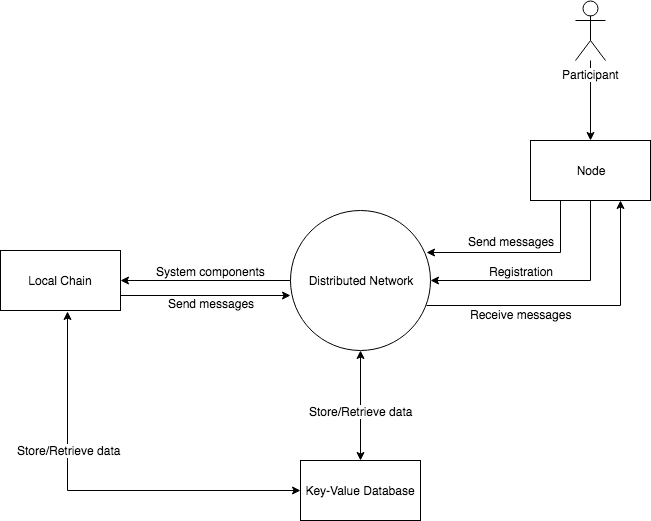
\includegraphics[width=0.7\textwidth]{Context_Diagram}
  \caption[Context Diagram] {
    Context Diagram waarin de interacties te zien is tussen het systeem en zijn omgeving.
  }
\end{figure}

De gebruiker draait een Node die gebruik maakt van het Peer-to-Peer netwerk om berichten te versturen. Een van de berichten is specifiek weergegeven aangezien het gaat om de registratie van een nieuwe gebruiker in het systeem. Het Distributed Network maakt gebruik van entiteiten uit de Local Chain om de benodigde data te versturen. 

Zowel het Local Chain gedeelte als het Distributed Network maken gebruik van een Key-Value database om data op te slaan. In het geval van het Distributed Network gaat dit om informatie over connecties.